%%
%% Copyright 2007, 2008, 2009 Elsevier Ltd
%%
%% This file is part of the 'Elsarticle Bundle'.
%% ---------------------------------------------
%%
%% It may be distributed under the conditions of the LaTeX Project Public
%% License, either version 1.2 of this license or (at your option) any
%% later version.  The latest version of this license is in
%%    http://www.latex-project.org/lppl.txt
%% and version 1.2 or later is part of all distributions of LaTeX
%% version 1999/12/01 or later.
%%
%% The list of all files belonging to the 'Elsarticle Bundle' is
%% given in the file `manifest.txt'.
%%

%% Template article for Elsevier's document class `elsarticle'
%% with numbered style bibliographic references
%% SP 2008/03/01
%%
%%
%%
%% $Id: elsarticle-template-num.tex 4 2009-10-24 08:22:58Z rishi $
%%
%%
\documentclass[preprint,10pt,5p]{elsarticle}
   
%% Use the option review to obtain double line spacing
%\documentclass[preprint,review,12pt]{elsarticle}

%% Use the options 1p,twocolumn; 3p; 3p,twocolumn; 5p; or 5p,twocolumn
%% for a journal layout:
%% \documentclass[final,1p,times]{elsarticle}
%% \documentclass[final,1p,times,twocolumn]{elsarticle}
%% \documentclass[final,3p,times]{elsarticle}
%% \documentclass[final,3p,times,twocolumn]{elsarticle}
%% \documentclass[final,5p,times]{elsarticle}
%% \documentclass[final,5p,times,twocolumn]{elsarticle}

%% if you use PostScript figures in your article
%% use the graphics package for simple commands
%% \usepackage{graphics}
%% or use the graphicx package for more complicated commands
%% \usepackage{graphicx}
%% or use the epsfig package if you prefer to use the old commands
%% \usepackage{epsfig}

%% The amssymb package provides various useful mathematical symbols
\usepackage{amssymb}
%% The amsthm package provides extended theorem environments
%% \usepackage{amsthm}

%% The lineno packages adds line numbers. Start line numbering with
%% \begin{linenumbers}, end it with \end{linenumbers}. Or switch it on
%% for the whole article with \linenumbers after \end{frontmatter}.
\usepackage{lineno}
\usepackage{amsmath}

\usepackage{amsmath}
\usepackage{algorithm}
\usepackage[noend]{algpseudocode}

%% Acrescentei o pacote abaixo para usar subfigures mas talvez não seja recomendado...
\usepackage{subcaption}

%% Acrescentei este pacote aqui para linhas duplas em tabelas sem cortes
\usepackage{hhline}

%% Acrescentei este pacote para permitir links clicáveis
\usepackage{hyperref}

%% natbib.sty is loaded by default. However, natbib options can be
%% provided with \biboptions{...} command. Following options are
%% valid:

%%   round  -  round parentheses are used (default)
%%   square -  square brackets are used   [option]
%%   curly  -  curly braces are used      {option}
%%   angle  -  angle brackets are used    <option>
%%   semicolon  -  multiple citations separated by semi-colon
%%   colon  - same as semicolon, an earlier confusion
%%   comma  -  separated by comma
%%   numbers-  selects numerical citations
%%   super  -  numerical citations as superscripts
%%   sort   -  sorts multiple citations according to order in ref. list
%%   sort&compress   -  like sort, but also compresses numerical citations
%%   compress - compresses without sorting
%%
%% \biboptions{comma,round}

% \biboptions{}

\usepackage{booktabs}


%% AQUI COMEÇA A PARTE EM QUE VOCÊ DEVE MEXER ...

\journal{Computers and Electronics in Agriculture}



\begin{document}

\begin{frontmatter}

\title{Evite Títulos Muito Longos e Destaque apenas o que é Mais Importante}

\address[label1]{Universidade Católica Dom Bosco, Campo Grande, Brazil}
\address[label2]{Universidade Federal de Mato Grosso do Sul, Campo Grande, Brazil}
\address[label3]{Universidade Estadual de Mato Grosso do Sul, Campo Grande, Brazil}

\author[label1]{Nome do Aluno que Mais Trabalhou no Projeto\corref{cor1}}
\ead{aluno@ucdb.br}
\cortext[cor1]{Corresponding author}

\author[label3]{Segundo Autor}
\ead{segundo@uems.br}

\author[label1]{Outros Autores}
\ead{segundo@uems.br}

%% 
\author[label1,label2]{Hemerson Pistori}
\ead{pistori@ucdb.br}


\begin{abstract}
Um único parágrafo resumindo o problema, a solução proposta, a metodologia usada para validar a proposta e o principal resultado. Um erro comum no resumo é falar muito mais do problema do que aquilo que você efetivamente fez. A maior parte do resumo tem que ser sobre a sua contribuição\end{abstract}

% The first keyword should be selected from the list of EJOR Keywords.
% Please include up to 4 additional keywords of your choice.

\begin{keyword}
palavra chave 1 \sep palavra 2 \sep palavra 3 \sep se possível use palavras-chave que não aparecem no título para aumentar as chances do artigo aparecer nas buscas automáticas

\end{keyword}


\end{frontmatter}


%%
%% Start line numbering here if you want
%%
%\linenumbers




%%%%%%%%%%%%%% I N T R O D U C A O %%%%%%%%%%%%%%%%%%%%%%%%%%%%%%%%%%%%%%%%%%%%%%%%%%%%%%%%%%%%%

\section{Introduction}
\label{intro}

A introdução deve oferecer uma visão geral sobre a área em que seu problema se insere (pecuária de precisão, piscicultura, criminalística, cana de açuar etc) e dizer qual é o problema específico que você busca resolver e porque resolver este problema é importante. Deve também fazer uma introdução resumida das outras seções do artigo: trabalhos correlatos, materiais e métodos, resultados e discussão. Opcionalmente, se não houver muitos trabalhos correlatos, dá para colocá-los na introdução, ao invés de criar uma seção específica para isso. Finalmente, a coisa mais importante da introdução é deixar muito claro quais são as principais contribuições deste artigo para o avanço da ciência (E.g.: novo banco de imagens, nova maneira de resolver um problema, avaliação de uma técnica existente em um novo problema, etc).
    
Aqui eu mostro dois exemplo de citação no Latex, uma com os autores fazendo parte da frase como sujeitos ou objetos e a outra com a citação ficando no final da frase. \citet{tola2010daisy} aplicaram a técnica Coisa para resolver o problema Cabeludo. Uma outra maneira de resolver o problema Cabeludo é através da técnica Outra Coisa Melhor~\cite{bouvier2008}. Note que o uso de \textit{citet} e \textit{cite} faz toda a diferença na formatação final. Com \textit{citet} além de colocar o número entre colchetes o Latex também coloca os autores.  A Figura~\ref{fig:rumicam} é um exemplo de como incluir uma imagem no artigo. Os arquivos das imagens estão na pasta \textit{figures}. 


\begin{figure}
  \centering
  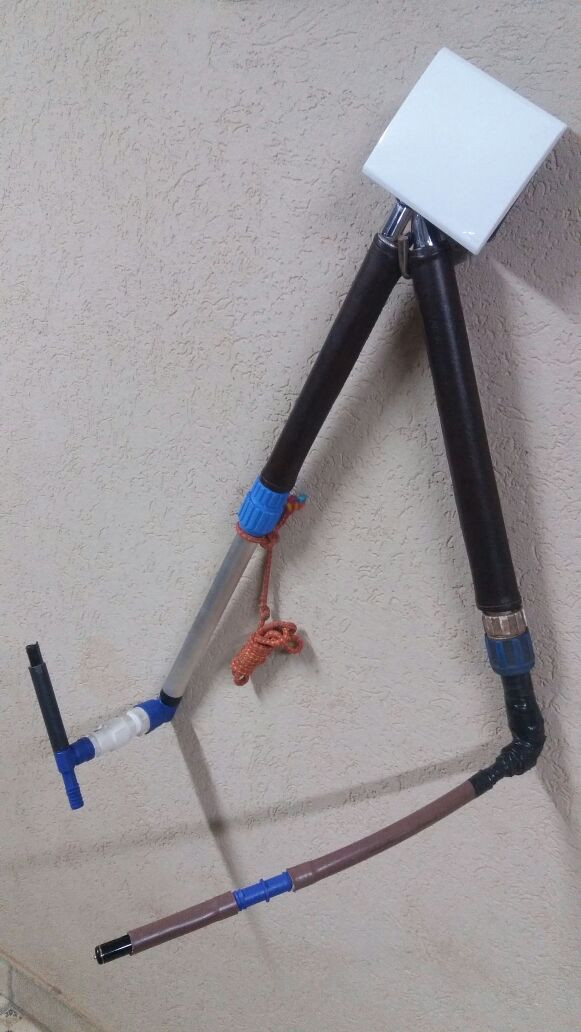
\includegraphics[width=0.4\linewidth]{figures/rumicam.jpg} 

   \caption{A descrição da figura precisa ser completa. O leitor tem que ser capaz de entender a figura mesmo sem ler o artigo.}
   \label{fig:rumicam}
\end{figure}
 
    


%%%%%%%%%%%%%%  R E L A T E D   W O R K S  %%%%%%%%%%%%%%%%%%%%%%%%%%%%%%%%%%%%%%%

\section{Related Works}
\label{works}

Citar trabalhos científicos recentes, publicados em In\-glês de preferência, que tenham relação com problemas iguais ou similares ao que você está tentando resolver ou trabalhos que aplicam as mesmas técnicas que você irá testar mas em outros problemas. A escolha deve ser sistemática e com critérios claros de inclusão e exclusão (ao invés de uma escolha aleatória de alguns artigos). Deve mostrar que está por dentro do que está acontecendo na área. Não é um simples resumo de cada artigo, um por parágrafo, mas parágrafos que ``costuram'' ou inter-relacio\-nam ideias presentes em vários artigos e as comparam com o seu próprio trabalho, indicando as diferenças que justificam mais este novo artigo que você está escrevendo. 




%%%%%%%%%%%%%%  M A T E R I A I S  E   M E T O D O S   %%%%%%%%%%%%%%%%%%%%%%%%%%%%%%%%%%%%%%%

\section{Materials and Methods}
\label{methods}

Em materiais e métodos você descreve as técnicas utilizadas, como foram combinadas e com quais configurações e parâmetros (E.g.: técnicas usadas para pré-processamento, extração de atributos, segmentação, regressão, contagem, aprendizagem automática, etc). Deve também descrever detalhadamente como foram feitos os experimentos (descrição do banco de imagens incluindo detalhes de como as imagens foram capturadas, métricas de desempenho, técnicas de amostragem como por exemplo a validação cruzada estratificada em 10 dobras, testes de hipótese e outras ferramentas descritivas como box-plots e matrizes de confusão). Você não irá mostrar aqui a matriz de confusão ou boxplots, por exemplo, apenas dizer que gerou uma ou várias durante o experimento. 

Sugestão de subseções para esta seção:

\subsection{Dataset}

Descrever aqui, em detalhes, como foi a coleta dos dados (datas, equipamentos, parâmetros, procedimentos, etc), como foram anotações, como ficou o banco de imagens final, etc. Mostrar alguns exemplos de imagens.

\subsection{Models}

Descrever aqui as técnicas ou modelos que foram utilizados

\subsection{Experimental Setup}

Descrever aqui como foi feito o experimento com as técnicas


%%%%%%%%%%%%%%  R E S U L T A D O S    %%%%%%%%%%%%%%%%%%%%%%%%%%%%%%%%%%%%%%%


\section{Results}

Aqui você mostra quais foram os resultados dos experimentos (números, tabelas, gráficos, valores-p, matriz de confusão, etc). A descrição textual das tabelas e gráficos, destacando alguns valores máximos e mínimos, também deve ficar aqui nesta seção. A tabela~\ref{table:expDeepLearning} é um exemplo de como incluir tabelas no artigo. É possível trazer a discussão para esta seção, que passaria a se chamar então \textit{Results and Discussion}.


\begin{table}[h!]
\centering
\caption{A legenda da tabela também precisa ser bem descritiva e explicar o que são as colunas e linhas e para que está sendo usado o negrito}
\label{table:expDeepLearning}
\begin{tabular}{|c|c|c|c|} 
   \hline
   Arquit.    & Precision               & Recall                  & F-Score \\ 
   \hline\hline
   VGG19      & 57 ($\pm$ 1.2)          & 52 ($\pm$ 3.3)          & 54.4 ($\pm$ 1.2)\\
   \hline
   VGG16      & 63 ($\pm$ 0.5)          & \textbf{63 ($\pm$ 2.1)} & 62.5 ($\pm$ 3.2)\\
   \hline
   Xception   & 60 ($\pm$ 3.3)          & 43 ($\pm$ 0.2)          & \textbf{70 ($\pm$ 2.1)} \\
   \hline
   ResNet50   & \textbf{69 ($\pm$ 5.2)} & 32 ($\pm$ 1.8)          & 43.7 ($\pm$ 1.8) \\
   \hline
\end{tabular}
\end{table}

Uma outra maneira de criar as tabelas é através deste editor: \href{https://www.tablesgenerator.com/}{CLIQUE AQUI}







%%%%%%%%%%%%%%  D I S C U S S Ã O %%%%%%%%%%%%%%%%%%%%%%

\section{Discussion}




Esta é a parte mais difícil de escrever pois é preciso aqui interpretar os resultados e tentar explicá-los ou justificá-los com base na literatura e nos dados obtidos. É a seção que mais precisa de criatividade e compreensão dos fundamentos, das técnicas, da estatística, dos trabalhos correlatos, etc. Aqui você terá que defender em quais pontos sua proposta tem vantagens em relação a outras alternativas e também identificar as deficiências. Também é preciso tentar explicar quais são os elementos que levam a técnica a errar. Uma coisa bem interessante para fazer aqui é mostrar imagens onde a técnica erra e discutir os motivos que podem estar levando ao erro (tentando explicar estes motivos com base no funcionamento da técnica ou em limitação do banco de imagens). Existe a possibilidade de juntar a seção de resultados com a discussão, como disse anteriormente,  principalmente se a discussão estiver muito curta (mas o melhor é tentar fazer uma boa discussão).Apenas dizer que o algoritmo X teve a maior acurácia ou medida-F não é discutir (isso é apenas o resultado escrito de outra forma e deve ir na seção de resultados mesmo).


É preciso muito cuidado na interpretação do valor-p. Neste link This is my link: \href{https://www.scielo.br/pdf/jbpneu/v41n5/pt_1806-3713-jbpneu-41-05-00485.pdf}{CLIQUE AQUI} para ver um texto falando dos erros comuns no uso do valor-p. Abaixo eu mostro dois exemplos de usos corretos:

Para valor-p baixo: ``Através do teste ANOVA chegou-se ao valor-p de .03 que indica uma diferença estatisticamente significativa no desempenho médio das técnicas testadas a um nível de significância de 5\% usando a medida-F como métrica'' 

Para valor-p alto: ``Através do teste ANOVA chegou-se ao valor-p de .25 e portanto não temos evidência de que exista uma diferença estatisticamente significativa no desempenho médio das técnicas testadas a um nível de significância de 5\% usando a medida-F como métrica'' 



A Figura~\ref{fig:second} é um exemplo de como incluir várias imagens lado a lado. Na imagem vemos duas vacas com a boca aberta (\ref{fig:sepopen} and~\ref{fig:novopen}) e duas com a boca fechada (\ref{fig:sepclo} and~\ref{fig:novclo}). 


\begin{figure}
  \centering
  \begin{subfigure}{0.2\textwidth}
    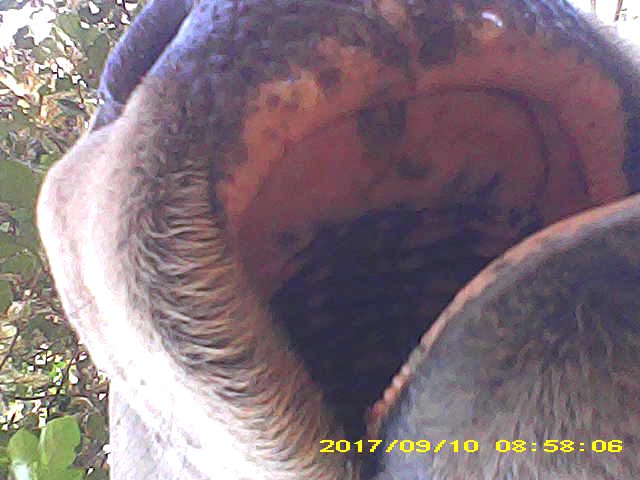
\includegraphics[width=1\linewidth]{figures/sep_open_caranelo.png} 
    \caption{Opened Caracu Hybrid}
    \label{fig:sepopen}
  \end{subfigure}
  \quad
  \begin{subfigure}{0.2\textwidth}
     
\includegraphics[width=1\linewidth]{figures/nov_open_nelore.png}
     \caption{Opened Nelore}
     \label{fig:novopen}
   \end{subfigure}
  \quad
  \begin{subfigure}{0.2\textwidth}
     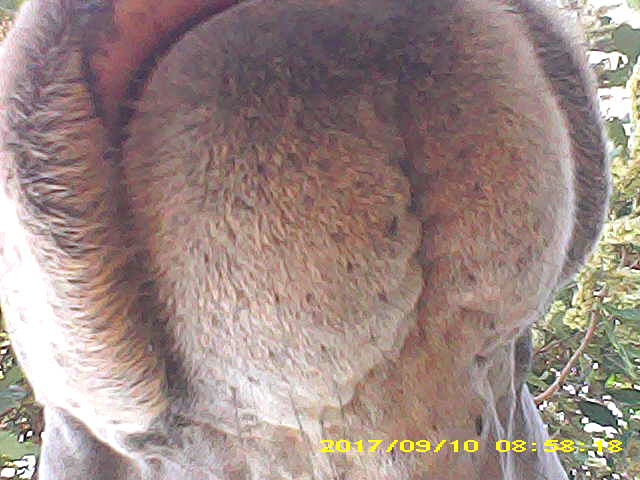
\includegraphics[width=1\linewidth]{figures/sep_closed_caranelo.png}
     \caption{Closed Caracu Hybrid}
     \label{fig:sepclo}
   \end{subfigure}
  \begin{subfigure}{0.2\textwidth}
     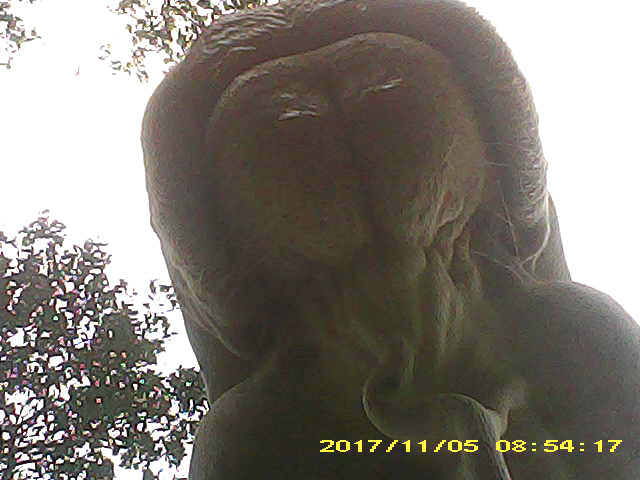
\includegraphics[width=1\linewidth]{figures/nov_closed_nelore.png}
     \caption{Closed Nelore}
     \label{fig:novclo}
   \end{subfigure}

   \caption{Two samples for each of the classes used in the second experiment, one for each different day of data collection (a) Caracu hybrid with the mouth opened, (b) Nelore with the mouth opened, (c) Caracu hybrid with the mouth closed, (d) Nelore with the mouth closed}
   \label{fig:second}
\end{figure}
 




%%%%%%%%%%%%%%  C O N C L U S O E S %%%%%%%%%%%%%%%%%%%%%%%%%%%%%%%%%%%%%%%%%%%%%

\section{Conclusion}

Quais as principais conclusões de tudo o que foi feito (pode ser um resumo da discussão, destacando aquilo que você considera mais relevante). Na conclusão não se deve acrescentar novos resultados ou dados. Também pode-se incluir informações sobre o que você acha que outros pesquisadores podem fazer a mais para continuar avançando na solução deste ou de outros problemas similares que você identificou durante o projeto (trabalhos futuros).




\section{Acknowledgments}
This work has received financial support from the Dom Bosco Catholic University and the Foundation for the Support and Development of Education, Science and Technology from the State of Mato Grosso do Sul, FUNDECT. Some of the authors have been awarded with Scholarships from the the Brazilian National Council of Technological and Scientific Development, CNPq and the Coordination for the Improvement of Higher Education Personnel, CAPES. We would also like to thank NVIDIA for providing the Titan X GPUs used in the experiments.

% ==============================================================

%% The Appendices part is started with the command \appendix;
%% appendix sections are then done as normal sections
% \appendix

% \section{Section in Appendix}
% \label{appendix-sec1}


%% References
%%
%% Following citation commands can be used in the body text:
%% Usage of \cite is as follows:
%%   \cite{key}         ==>>  [#]
%%   \cite[chap. 2]{key} ==>> [#, chap. 2]
%%

%% References with bibTeX database:
% \bibliographystyle{elsarticle-num}
\bibliographystyle{elsarticle-harvard}


\bibliography{references}


\end{document}

